\usetikzlibrary{arrows}

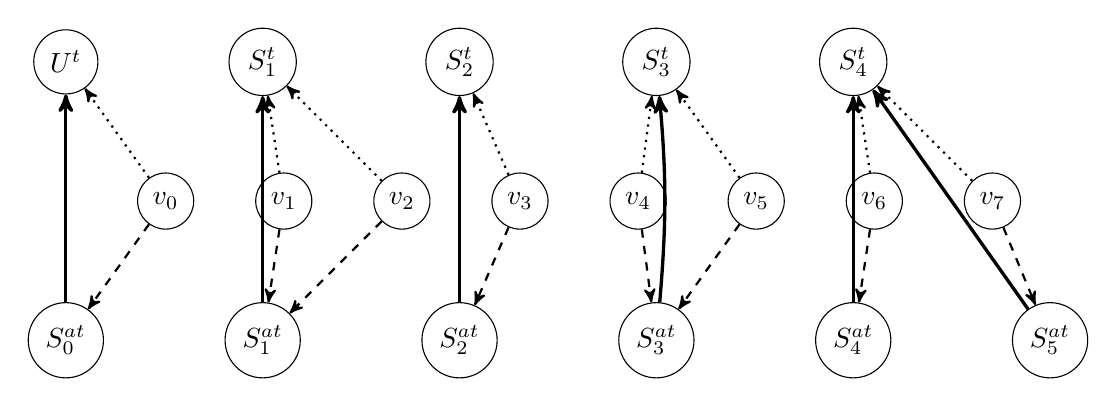
\begin{tikzpicture}[->,>=stealth',node distance=1.5cm,tnode/.style={node distance=2.5cm,draw,circle}]

\node[draw,circle] (0) {$v_0$};
\node[draw,circle,right of = 0] (1) {$v_1$};
\node[draw,circle,right of = 1] (2) {$v_2$};
\node[draw,circle,right of = 2] (3) {$v_3$};
\node[draw,circle,right of = 3] (4) {$v_4$};
\node[draw,circle,right of = 4] (5) {$v_5$};
\node[draw,circle,right of = 5] (6) {$v_6$};
\node[draw,circle,right of = 6] (7) {$v_7$};

\node[tnode,below left of = 0,xshift=.5cm] (ath0) {$S^{at}_0$};
\node[tnode,right of = ath0] (ath1) {$S^{at}_1$};
\node[tnode,right of = ath1] (ath2) {$S^{at}_2$};
\node[tnode,right of = ath2] (ath3) {$S^{at}_3$};
\node[tnode,right of = ath3] (ath4) {$S^{at}_4$};
\node[tnode,right of = ath4] (ath5) {$S^{at}_5$};

\node[tnode,above left of = 0,xshift=.5cm] (th0) {$\mathfrak{U}^t$};
\node[tnode,draw,circle,right of = th0] (th1) {$S^{t}_1$};
\node[tnode,draw,circle,right of = th1] (th2) {$S^{t}_2$};
\node[tnode,draw,circle,right of = th2] (th3) {$S^{t}_3$};
\node[tnode,draw,circle,right of = th3] (th4) {$S^{t}_4$};

\path
(0) edge[thick,dashed] (ath0)
(1) edge[thick,dashed] (ath1)
(2) edge[thick,dashed] (ath1)
(3) edge[thick,dashed] (ath2)
(4) edge[thick,dashed] (ath3)
(5) edge[thick,dashed] (ath3)
(6) edge[thick,dashed] (ath4)
(7) edge[thick,dashed] (ath5)

(0) edge[thick,dotted] (th0)
(1) edge[thick,dotted] (th1)
(2) edge[thick,dotted] (th1)
(3) edge[thick,dotted] (th2)
(4) edge[thick,dotted] (th3)
(5) edge[thick,dotted] (th3)
(6) edge[thick,dotted] (th4)
(7) edge[thick,dotted] (th4)

(ath0) edge[very thick] (th0)
(ath1) edge[very thick] (th1)
(ath2) edge[very thick] (th2)
(ath3) edge[very thick,bend right=5] (th3)
(ath4) edge[very thick] (th4)
(ath5) edge[very thick] (th4)
;
\end{tikzpicture}